\chapter{绪论}\label{introduction}

本章是对本文内容的简要说明,将先从电子表格,及其公式错误两方面介绍本文的研究背景,然后从研究问题、研究思路、研究贡献三方面介绍本文工作,最后对全文的组织结构进行说明。

\section{研究背景}

\subsection{电子表格及其用法}
电子表格是用于组织、分析和存储表格形式的数据的计算机应用程序。
尽管它们最初是为会计或簿记任务而开发的,但现在已广泛用于构建,排序和共享表格列表的任何环境。

电子表格对在表格的单元格中输入的数据进行操作。
每个单元格可以包含数字或文本数据,也可以包含基于其他单元格的内容自动计算并显示值的公式的结果。
电子表格也可以引用一个这样的电子文档。电子表格用户可以调整任何存储的值,并观察对计算值的影响。
这使得电子表格可用于“假设分析”,因为无需手动重新计算即可快速调查许多情况。
现代电子表格软件可以具有多个交互工作表,并且可以以文本和数字或图形形式显示数据。

除了执行基本的算术和数学功能外,现代电子表格还提供了用于常见财务会计和统计操作的内置功能。
这样的计算如净现值或标准偏差可以应用于表格数据与在公式中的预编程的功能。
电子表格程序还提供条件表达式,在文本和数字之间转换的函数以及对文本字符串进行操作的函数。

\begin{figure}[t!]
    \centering
    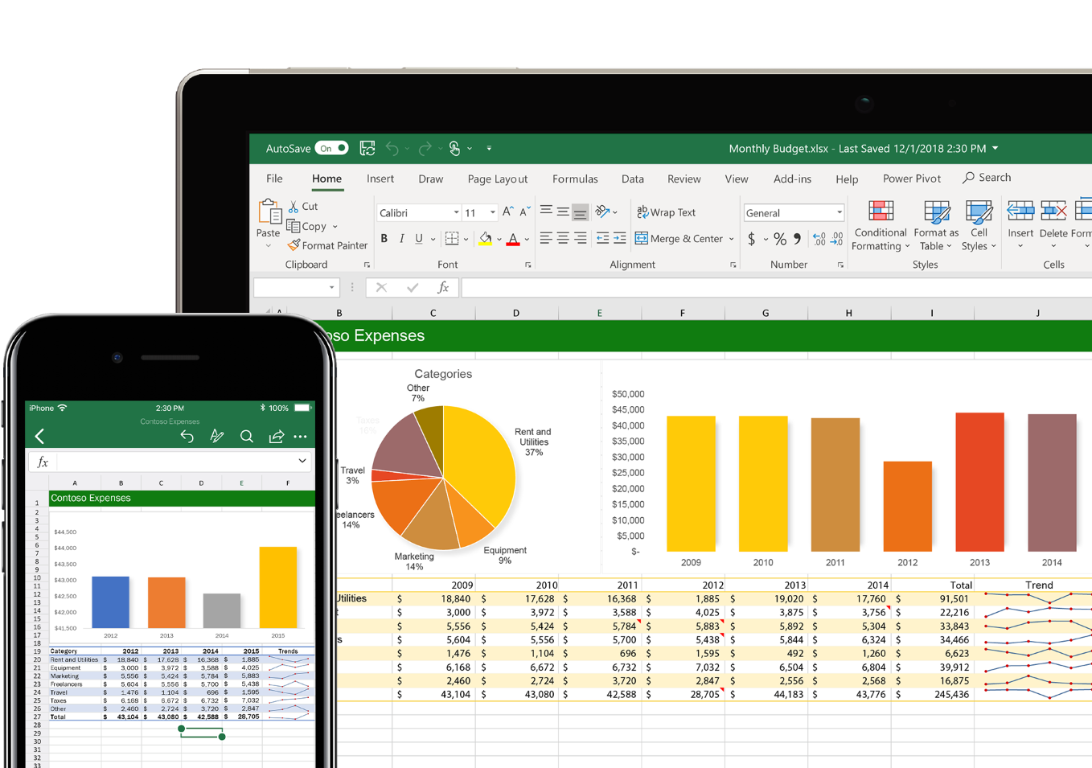
\includegraphics[width=0.6\textwidth]{figures/figure1.png}
    \caption{Microsoft Excel Spreadsheet Software}   
    \label{fig:1} 
\end{figure}

电子表格已在整个商业环境中取代了基于纸张的系统。
如图所示,Microsoft Excel现在在Windows和Macintosh平台上拥有最大的市场份额。
电子表格程序是办公室生产力套件的标准功能; 自从Web应用程序问世以来,办公套件现在也以Web应用程序形式存在。
基于Web的电子表格是一个相对较新的类别。



\subsection{公式错误}


\section{本文工作}


\subsection{研究问题}


\subsection{研究思路}


\subsection{研究贡献}


\section{论文组织结构}

